

\documentclass[a4paper]{article}

\usepackage{amsmath}
\usepackage{hyperref}
\usepackage{biblatex}
\usepackage{enumerate}
\usepackage{graphicx}
\usepackage{stmaryrd}
\usepackage{listings}

\addbibresource{refs.bib}

\begin{document}

\author{Ola Bratt \\
  \href{mailto:ola.bratt@gmail.com}{ola.bratt@gmail.com}
}
\title{DAT565/DIT407 Assignment 1}
\date{2024-01-16}

\maketitle



\section*{Problem 1: Dependency Ratio}

Results are presented in Figure~\ref{fig:ratio} and
Figure~\ref{fig:fractions}.



\begin{figure}[h]
  \begin{center}
    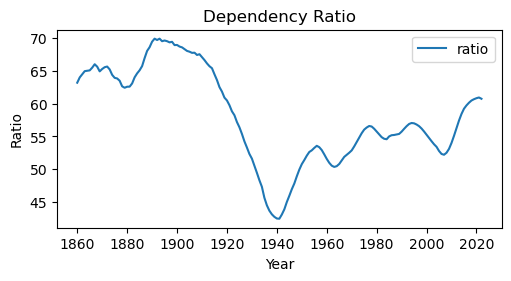
\includegraphics[width=\textwidth]{ratio.png}
    \caption{Dependecy ratio}
    \label{fig:ratio}
  \end{center}
\end{figure}

\newpage
If you need to cite external sources, do so by placing the literature
assignment, we use data from SCB~\cite{SCB:2023}.

\begin{figure}[h]
  \begin{center}
    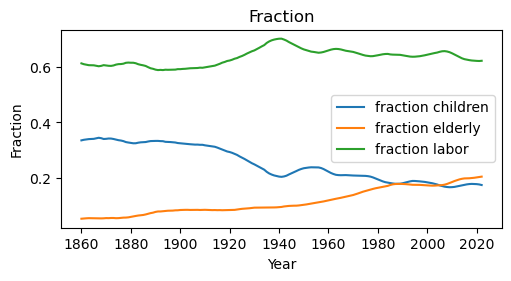
\includegraphics[width=\textwidth]{fractions.png}
    \caption{Fractions}
    \label{fig:fractions}
  \end{center}
\end{figure}


Discussion of results.

\printbibliography

\section*{Appendix: Source Code}
\lstinputlisting{assignment1.ipynb}

\end{document}
